\documentclass[10pt]{report}

\usepackage{verbatim}
\usepackage{subcaption} % for subfigures
%\usepackage{amsthm} % for QED
%\usepackage{algpseudocode} % for pseudo-code
\usepackage{mathtools} % for \xRightarrow

\usepackage{listings} % for code
\lstset
{
	language=Matlab,
	frame=single,
	basicstyle=\footnotesize,
	numbers=left,
	stepnumber=1,
	showstringspaces=false,
	tabsize=4,
	breaklines=true,
	breakatwhitespace=false,
}

\usepackage{siunitx} % for scientific notation
% for `e' in scientific notation
\sisetup{output-exponent-marker=\ensuremath{\mathrm{e}}}

\usepackage{float} % for figure [H]
\usepackage{booktabs} % for tabular
\usepackage{caption} % for \caption*
\usepackage[export]{adjustbox} % for valign=t
\usepackage{array} % for column type m
\usepackage{verbatim}
\usepackage{graphicx}
\graphicspath{ {imgs/} }
\usepackage{fancyhdr}
\usepackage{amssymb}
\usepackage{amsmath}

%%%%%% Pagination
\setlength{\topmargin}{-.3 in}
\setlength{\oddsidemargin}{0in}
\setlength{\evensidemargin}{0in}
\setlength{\textheight}{9.in}
\setlength{\textwidth}{6.5in}

%Title page
\newcommand{\hwTitle}{Homework \#3}
\newcommand{\hwCourse}{Introduction to Computational Mathematics}
\newcommand{\hmwkClassInstructor}{Professor Shuwang Li}

\title{
	\vspace{2in}
	\textmd{\textbf{\hwCourse\\\hwTitle}}\\
	\vspace{0.3in}\large{\textit{\hmwkClassInstructor}}
	\vspace{3in}
}

%\title{Homework 1}
\author{\textbf{Zhihao Ai}}
\date{}

%Header setting.
\pagestyle{fancy}
\fancyhead[L]{Zhihao Ai}
\fancyhead[C]{Math 350}
\fancyhead[R]{Homework 3}
%%%%%%

%\displaystyle apply to all
\everymath{\displaystyle}

%Custom commands.
\newcommand{\ds}{\displaystyle}
\newcommand{\eva}[2] {\left. #1 \right|_{#2}}
\newcommand{\dintt}[4] {\int_{#1}^{#2} #3 d#4}

\newcolumntype{C}{ >{\centering\arraybackslash} m{3em} }
\newcolumntype{D}{ >{\centering\arraybackslash} m{4em} }
\newcolumntype{N}{ >$ c <$}

\newcommand{\abs}[1] {\left| #1 \right|}
\newcommand{\norm}[2][\infty] {\left\Vert \mathbf{#2} \right\Vert_#1}

\begin{document}

\maketitle

\section*{Part 1. Reading Assignment}

\section*{Part 2. Fundamental Concepts/Ideas}
\begin{enumerate}
	\item 
	The exact solution to the following linear system is $\mathbf{x} = (1, -2, 3)^\mathrm{T}$.
	\begin{align*}
		10x_1 - 2x_2 - x_3 &= 11\\
		-2x_1 + 10x_2 - x_3 &= -25\\
		-x_1 - 2x_2 + 5x_3 &= 18
	\end{align*}
	\begin{enumerate}
		\item 
		Solve the system using Gauss--Jacobi iterative method with $\mathbf{x}^{(0)} = (0, 0, 0)^\mathrm{T}$, stop the iteration if tolerance, $tol = \norm{x^{(\mathit k + \mathrm 1)} - x^{(\mathit{k})}} \le 0.5\times 10^{-2}$
		
		According to the coefficient matrix,
		\begin{align*}
			M &= -D^{-1}(A-D) = -\begin{pmatrix}
			0.1 & 0 & 0\\
			0 & 0.1 & 0\\
			0 & 0 & 0.2
			\end{pmatrix}
			\begin{pmatrix}
			0 & -2 & -1\\
			-2 & 0 & -1\\
			-1 & -2 & 0
			\end{pmatrix}
			=
			\begin{pmatrix}
			0 & 0.2 & 0.1\\
			0.2 & 0 & 0.1\\
			0.2 & 0.4 & 0
			\end{pmatrix}
			\\
			\mathbf{g} &= D^{-1}\mathbf{b} = \begin{pmatrix}
			0.1 & 0 & 0\\
			0 & 0.1 & 0\\
			0 & 0 & 0.2
			\end{pmatrix}
			\begin{pmatrix}
			11\\
			-25\\
			18
			\end{pmatrix}
			=
			\begin{pmatrix}
			1.1\\
			-2.5\\
			3.6
			\end{pmatrix}
		\end{align*}
		Apply $\mathbf{x}^{(k)} = M\mathbf{x}^{(k-1)} + \mathbf{g}$ iteratively with $\mathbf{x}^{(0)} = (0, 0, 0)^\mathrm{T}$ using Matlab:
		\lstinputlisting{hw3p1a.m}
		The code above produces:
		\begin{table}[H]
			\centering
			\begin{tabular}{NNN} \toprule
				k & x^{(k)} & tol \\ \midrule
				1 & (1.1000,-2.5000,3.6000)^\mathrm{T} & 3.6000\\
				2 & (0.9600,-1.9200,2.8200)^\mathrm{T} & 0.7800\\
				3 & (0.9980,-2.0260,3.0240)^\mathrm{T} & 0.2040\\
				4 & (0.9972,-1.9980,2.9892)^\mathrm{T} & 0.0348\\
				5 & (0.9993,-2.0016,3.0002)^\mathrm{T} & 0.0110\\
				6 & (0.9997,-2.0001,2.9992)^\mathrm{T} & 0.0015\\
				\bottomrule
			\end{tabular}
		\end{table}
		
		\item 
		Solve the system using Gauss--Seidel iterative method with $\mathbf{x}^{(0)} = (0, 0, 0)^\mathrm{T}$, stop the iteration if tolerance, $tol = \norm{x^{(\mathit k + \mathrm 1)} - x^{(\mathit{k})}} \le 0.5\times 10^{-2}$
		
		According to the coefficient matrix,
		\begin{align*}
		M &= -(L+D)^{-1}U = -\begin{pmatrix}
		0.1 & 0 & 0\\
		0.02 & 0.1 & 0\\
		0.028 & 0.04 & 0.2
		\end{pmatrix}
		\begin{pmatrix}
		0 & -2 & -1\\
		0 & 0 & -1\\
		0 & 0 & 0
		\end{pmatrix}
		=
		\begin{pmatrix}
		0 & 0.2 & 0.1\\
		0 & 0.04 & 0.12\\
		0 & 0.056 & 0.068
		\end{pmatrix}
		\\
		\mathbf{g} &= (L+D)^{-1}\mathbf{b} = \begin{pmatrix}
		0.1 & 0 & 0\\
		0.02 & 0.1 & 0\\
		0.028 & 0.04 & 0.2
		\end{pmatrix}
		\begin{pmatrix}
		11\\
		-25\\
		18
		\end{pmatrix}
		=
		\begin{pmatrix}
		1.1\\
		-2.28\\
		2.908
		\end{pmatrix}
		\end{align*}
		Apply $\mathbf{x}^{(k)} = M\mathbf{x}^{(k-1)} + \mathbf{g}$ iteratively with $\mathbf{x}^{(0)} = (0, 0, 0)^\mathrm{T}$ using Matlab:
		\lstinputlisting{hw3p1b.m}
		The code above produces:
		\begin{table}[H]
			\centering
			\begin{tabular}{NNN} \toprule
				k & x^{(k)} & tol \\ \midrule
				1 & (1.1000,-2.2800,2.9080)^\mathrm{T} & 2.9080\\
				2 & (0.9348,-2.0222,2.9781)^\mathrm{T} & 0.2578\\
				3 & (0.9934,-2.0035,2.9973)^\mathrm{T} & 0.0586\\
				4 & (0.9990,-2.0005,2.9996)^\mathrm{T} & 0.0057\\
				5 & (0.9999,-2.0001,2.9999)^\mathrm{T} & 0.0008\\
				\bottomrule
			\end{tabular}
		\end{table}
		
		\item 
		Interchange equation \#2 and \#3, do (a) and (b).
		
		Applying \verb|A = A([1 3 2],:)| to each of the code above, we get
		\begin{table}[H]
			\centering
			\begin{tabular}{NNN} \toprule
				k & x^{(k)} & tol \\ \midrule
				1 & (1.1000,12.5000,-18.0000)^\mathrm{T} & 18.0000\\
				2 & (1.8000,-33.0500,104.8000)^\mathrm{T} & 122.8000\\
				3 & (4.9700,273.6000,-352.1000)^\mathrm{T} & 456.9000\\
				4 & (20.6100,-870.2350,2708.0600)^\mathrm{T} & 3060.1600\\
				5 & (97.8590,6772.3450,-8761.5700)^\mathrm{T} & 11469.6300\\
				\vdots & \vdots & \vdots\\
				\bottomrule
			\end{tabular}
			\caption*{$x^{(\mathrm{k})}$ using Gauss--Jacobi iterative method}
			\hfill\\
			\begin{tabular}{NNN} \toprule
				k & x^{(k)} & tol \\ \midrule
				1 & (1.1000,11.9500,99.3000)^\mathrm{T} & 99.3000\\
				2 & (13.4200,254.0400,2495.5600)^\mathrm{T} & 2396.2600\\
				3 & (301.4640,6100.6680,60385.7520)^\mathrm{T} & 57890.1920\\
				4 & (7259.8088,147346.9756,1458932.1384)^\mathrm{T} & 1398546.3864\\
				5 & (175363.7090,3559660.9915,35245864.4973)^\mathrm{T} & 33786932.3589\\
				\vdots & \vdots & \vdots\\
				\bottomrule
			\end{tabular}
			\caption*{$x^{(\mathrm{k})}$ using Gauss--Seidel iterative method}
		\end{table}
		
		\item 
		What can you learn from this problem?
		
		In part (a), the coefficient matrix is diagonally dominant and $\norm[2]{M} < 1$:
		\[
		M^\mathrm{T}M = \begin{pmatrix}
		0.08 & 0.08 & 0.02\\
		0.08 & 0.2 & 0.02\\
		0.02 & 0.02 & 0.02
		\end{pmatrix}, 
		\rho(M^\mathrm{T}M) \approx 0.2432
		\to \norm[2]{M} = \sqrt{\rho(M^\mathrm{T}M)} \approx 0.4932 < 1
		\]
		When equation \#2 and \#3 are interchanged, the matrix is not diagonally dominant and $\norm[2]{M} > 1$:
		\[
		M^\mathrm{T}M = \begin{pmatrix}
		4.25 & -20 & -1.25\\
		-20 & 100.04 & 0.02\\
		-1.25 & 0.02 & 6.26
		\end{pmatrix}, 
		\rho(M^\mathrm{T}M) \approx 104.05
		\to \norm[2]{M} = \sqrt{\rho(M^\mathrm{T}M)} \approx 10.2 > 1
		\]
		In part (b), the coefficient matrix is diagonally dominant and $\norm[2]{M} < 1$:
		\[
		M^\mathrm{T}M \approx \begin{pmatrix}
		0 & 0 & 0\\
		0 & 0.0448 & 0.0286\\
		0 & 0.0286 & 0.0290
		\end{pmatrix}, 
		\rho(M^\mathrm{T}M) \approx 0.0665
		\to \norm[2]{M} = \sqrt{\rho(M^\mathrm{T}M)} \approx 0.2580 < 1
		\]
		When equation \#2 and \#3 are interchanged, the matrix is not diagonally dominant and $\norm[2]{M} > 1$:
		\[
		M^\mathrm{T}M \approx \begin{pmatrix}
		0 & 0 & 0\\
		0 & 2.01 & -34.245\\
		0 & -34.245 & 596.5
		\end{pmatrix}, 
		\rho(M^\mathrm{T}M) \approx 598.47
		\to \norm[2]{M} = \sqrt{\rho(M^\mathrm{T}M)} \approx 24.46 > 1
		\]
		We can see that if $A$ is diagonally dominant and $\norm[2]{M} < 1$, the iterative formula converges and $\lim\limits_{k\to \infty} \left\Vert \mathbf{x}^{(k)} - \mathbf{x} \right\Vert$ = 0, where $\mathbf{x}$ is the exact solution to $A\mathbf{x} = \mathbf{b}$; if not, $\mathbf{x}^{(k)}$ would not converge to the exact solution as shown in part (c). In addition, by comparing $\mathbf{x}^{(k)}$ produced by both methods, we conclude that $\mathbf{x}^{(k)}$ by Gauss--Seidel method converges faster than that by Gauss--Jacobi method.
		
	\end{enumerate}

	\item 
	Given $\sin(0.32)=0.314567, \sin(0.34)=0.333487, \sin(0.36)=0.352274$. Compute $\sin(0.3367)$ by Lagrange interpolation polynomial.
	\begin{enumerate}
		\item 
		A linear interpolation using the first two points.
		\begin{align*}
			l_0(x) &= \frac{x-0.34}{0.32-0.34},
			l_1(x) = \frac{x-0.32}{0.34-0.32}\\
			p_1(x) &= l_0(x)\cdot 0.314567 + l_1(x)\cdot 0.333487\\
			&\approx 0.946x + 0.011847\\
			p_1(0.3367) &\approx 0.330365
		\end{align*}
		
		\item 
		A quadratic interpolation using all three points.
		\begin{align*}
		l_0(x) &= \frac{(x-0.34)(x-0.36)}{(0.32-0.34)(0.32-0.36)},\\
		l_1(x) &= \frac{(x-0.32)(x-0.36)}{(0.34-0.32)(0.34-0.36)},\\
		l_2(x) &= \frac{(x-0.32)(x-0.34)}{(0.36-0.32)(0.36-0.34)}\\
		p_2(x) &= l_0(x)\cdot 0.314567 + l_1(x)\cdot 0.333487 + l_2(x)\cdot 0.352274\\
		&\approx -0.16625x^2 + 1.05573x - 0.006241\\
		p_2(0.3367) &\approx 0.330374
		\end{align*}
		
		\item 
		Estimate the absolute error in part (a) and (b).
		\begin{align*}
			\epsilon_a &= \abs{\sin{(0.3367)} - p_1(0.3367)} \approx 8.992\times 10^{-6}\\
			\epsilon_b &= \abs{\sin{(0.3367)} - p_2(0.3367)} \approx 1.705\times 10^{-7}
		\end{align*}
	\end{enumerate}
	\textit{Things learned}: Lagrange interpolation polynomial is able to give fairly good approximation of $f(x)$ on a certain interval. Even though higher order polynomial would lead to Runge's phenomenon near the edges, it produces generally better approximations around the center than polynomials with lower degrees, especially for $x$ that is close to $x_i$.
\end{enumerate}

\section*{Part 3. Computer Assignments}
\begin{enumerate}
	\item 
	Problem 3.3(a)(b) @ Page 19
	\begin{enumerate}
		\item
		Interpolate these data by each of the four interpolants discussed in this
		chapter: \verb|piecelin|, \verb|polyinterp|, \verb|splinetx|, and \verb|pchiptx|. Plot the results for $-1 \le x \le 1$.
		\begin{table}[H]
			\centering
			\begin{tabular}{*{7}{N}} \toprule
				x & -1.00 & -0.96 & -0.65 & 0.10 & 0.40 & 1.00\\ \midrule
				y & -1.0000 & -0.1512 & 0.3860 & 0.4802 & 0.8838 & 1.0000\\
				\bottomrule
			\end{tabular}
		\end{table}
		\lstinputlisting{hw3pa1.m}
		The script above produces:
		\begin{figure}[ht]
			\vspace{-2ex}
			\begin{subfigure}[b]{0.5\linewidth}
				\centering
				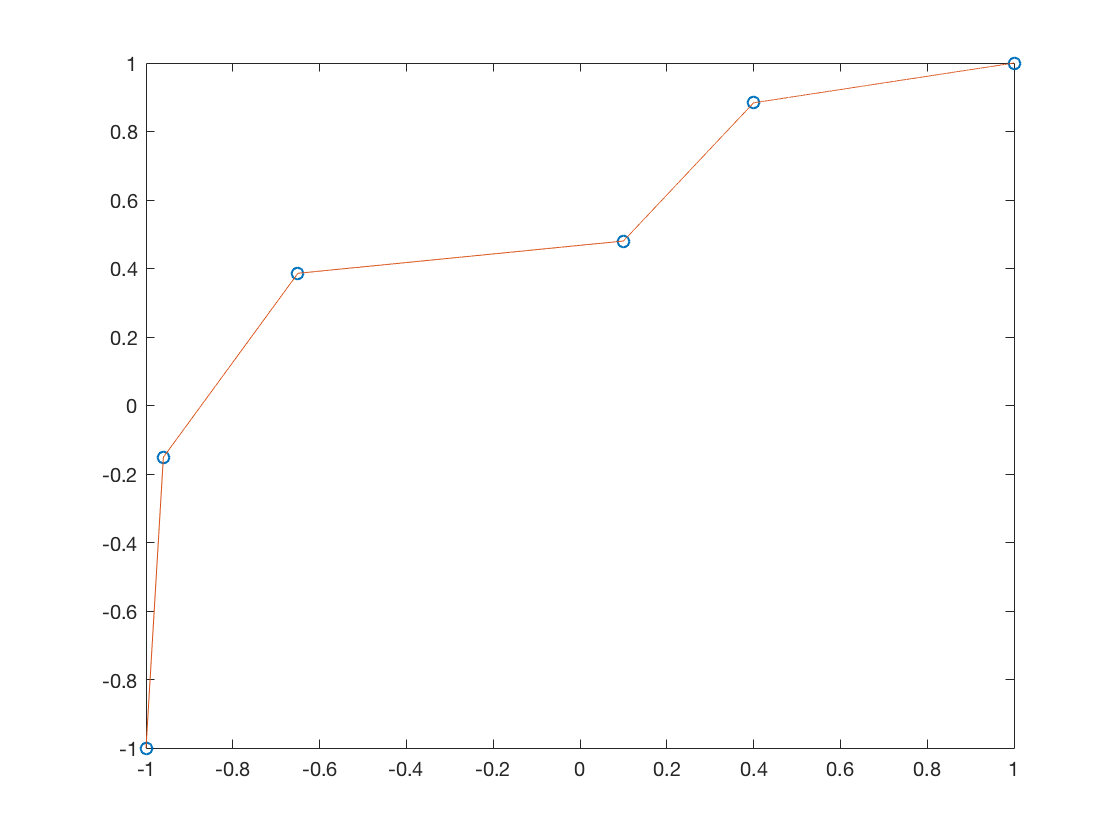
\includegraphics[width=\linewidth]{piecelin.png}
				\vspace{-5ex} 
				\caption*{\texttt{piecelin}}
			\end{subfigure}
			\begin{subfigure}[b]{0.5\linewidth}
				\centering
				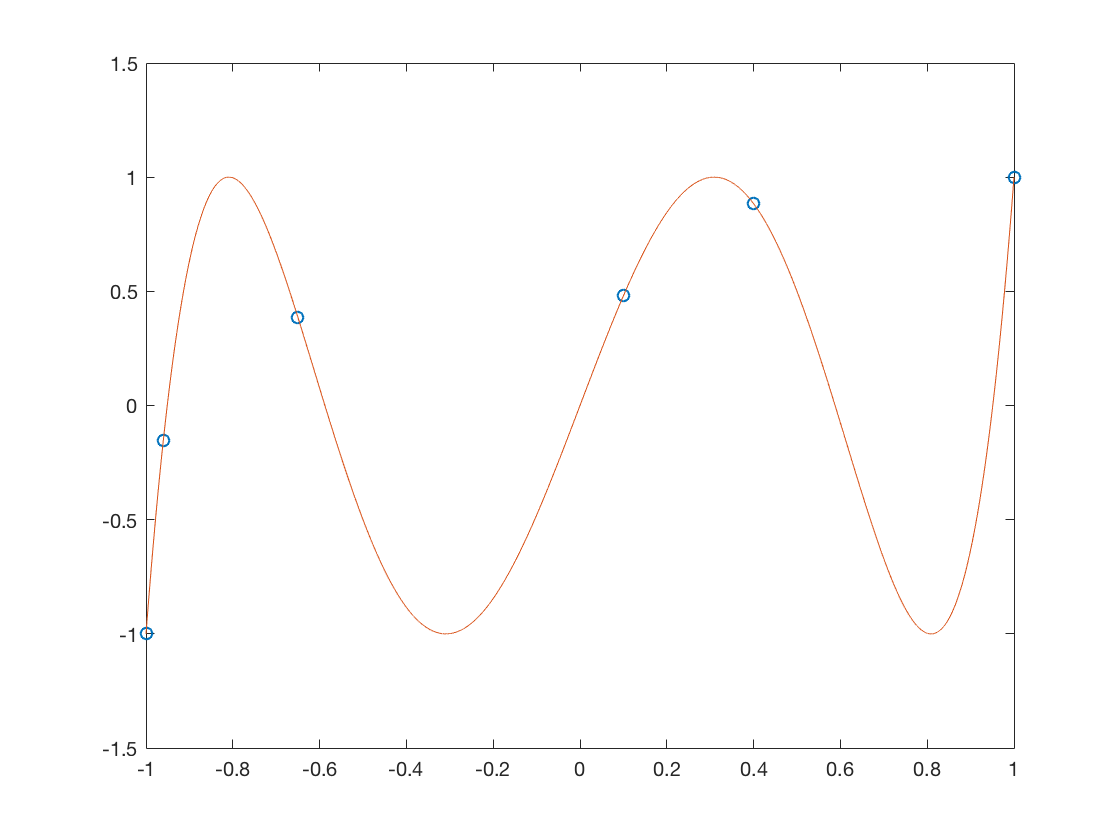
\includegraphics[width=\linewidth]{polyinterp.png} 
				\vspace{-5ex}
				\caption*{\texttt{polyinterp}}
			\end{subfigure}
			\begin{subfigure}[b]{0.5\linewidth}
				\centering
				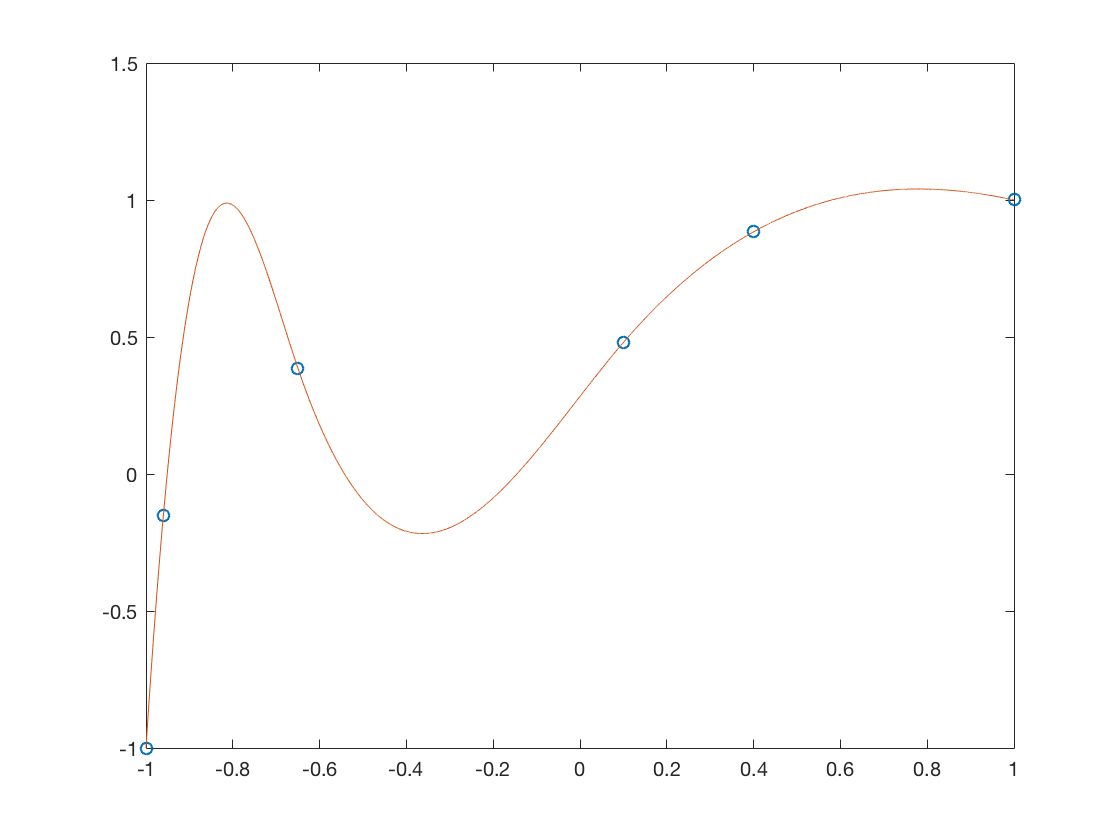
\includegraphics[width=\linewidth]{splinetx.png} 
				\vspace{-5ex}
				\caption*{\texttt{splinetx}}
			\end{subfigure}
			\begin{subfigure}[b]{0.5\linewidth}
				\centering
				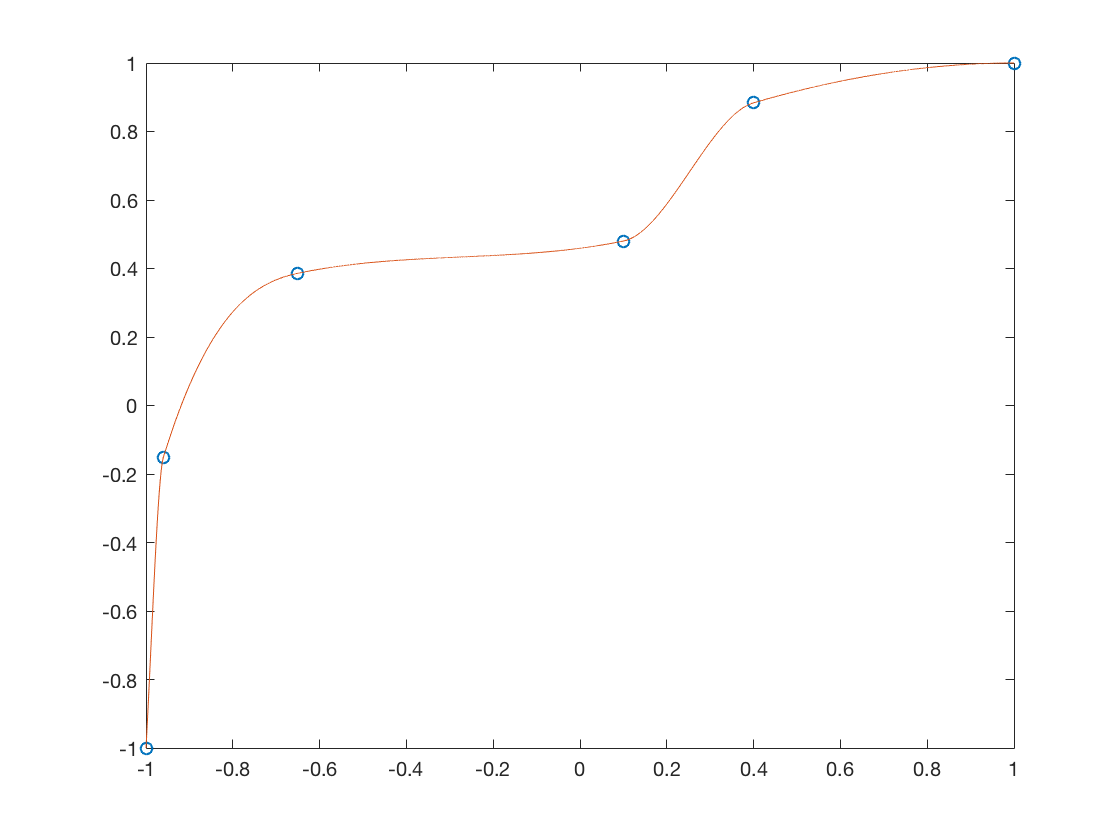
\includegraphics[width=\linewidth]{pchiptx.png} 
				\vspace{-5ex}
				\caption*{\texttt{pchiptx}}
			\end{subfigure} 
		\end{figure}
	
		\item 
		What are the values of each of the four interpolants at $x = -0.3$? Which
		of these values do you prefer? Why?
		
		\verb|piecelin|: $0.4300$; \verb|polyinterp|: $-0.9990$; \verb|splinetx|: $-0.1957$; \verb|pchiptx|: $0.4322$. I prefer $0.4322$ the most because for $-0.65<-0.3<0.10$, $y(-0.65)<0.4322<y(0.10)$. It preserves the  monotonicity and is much smoother than \verb|piecelin|.
	\end{enumerate}
	
	\item 
	Problem 3.4 @ Page 20
	\begin{enumerate}
		\item 
		Interpolate both functions of $x$ and $y$ on a finer grid and plot the result with \verb|splinetx|. Do the same thing with \verb|pchiptx|. Which do you prefer?
		\begin{figure}[H]
			\vspace{-2ex}
			\begin{subfigure}[b]{0.5\linewidth}
				\centering
				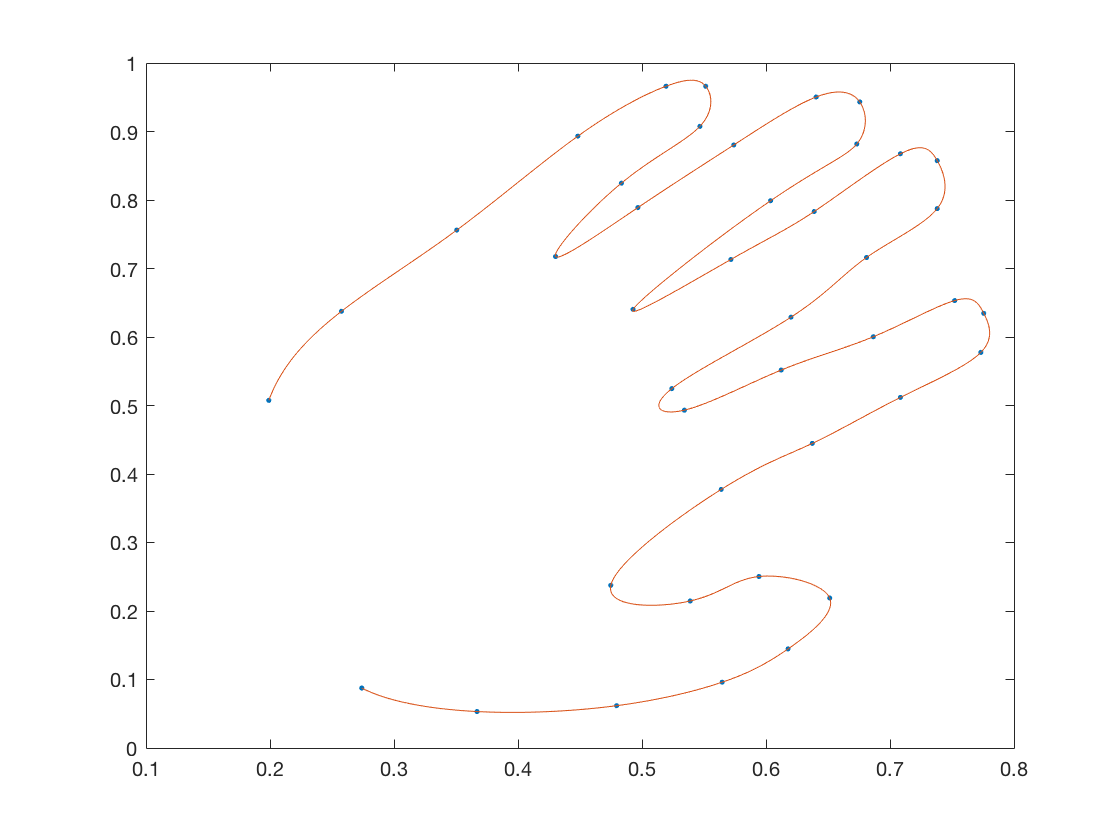
\includegraphics[width=\linewidth]{hand_splinetx.png}
				\vspace{-5ex} 
				\caption*{\texttt{splinetx}}
			\end{subfigure}
			\begin{subfigure}[b]{0.5\linewidth}
				\centering
				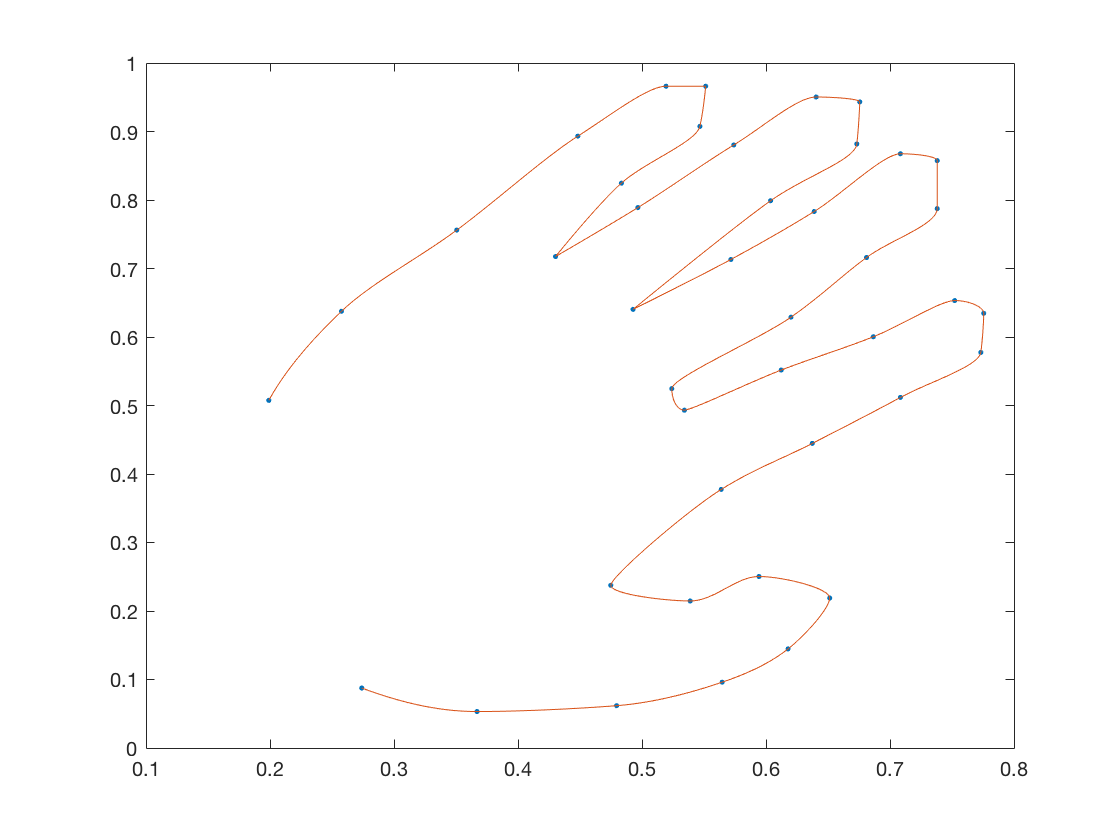
\includegraphics[width=\linewidth]{hand_pchiptx.png} 
				\vspace{-5ex}
				\caption*{\texttt{pchiptx}}
			\end{subfigure}
		\end{figure}
		I would prefer the one using \verb|splinetx| because it's much smoother than the other one.
		
		\item 
		Can you tell if Figure 3.11 was done with \verb|splinetx| or \verb|pchiptx|?
		
		It was done with \verb|splinetx|.
	\end{enumerate}
\end{enumerate}

\end{document}


